\chapter{Scelte progettuali}
\label{chap:scelte_progettuali}
Dato che Git è il sistema di versioning più utilizzato dagli sviluppatori di software\cite{gitmostused}, si è deciso di ispirarsi al suo modello di funzionamento per la realizzazione del primo VCS a grafi, chiamato \texttt{GGit}.
\section{Strutture dati di GGit}
\label{sec:strutture_dati}
Git è nato come un semplice content-addressable filesystem, ovvero un sistema di storage basato suuna relazione chiave-valore, nel quale è possibile archiviare qualsiasi tipo di contenuto digitale.Essenzialmente, l'azione di base che Git esegue è quella di memorizzare i contenuti di un file associandoli ad un hash calcolato su di essi: questa è la chiave che può essere utilizzata per accedere ai dati salvati.

L'hash di ogni oggetto (nomenclatura utilizzata per file e altre entità descritte in seguito), è calcolato usando l'algoritmo SHA-1, una funzione di hashing che genera un hash di 20 byte.
Pur essendo un algoritmo di hashing crittografico, SHA-1 non è sicuro, in quanto è stato provato che è possibile generare collisioni\cite{sha1collision} (ovvero due input che generano lo stesso hash).
Tuttavia, per l'utilizzo al quale è destinato all'interno di un VCS (cioè identificare univocamente il contenuto di un file) la complessità di SHA-1 è sufficiente, in quanto, nel peggior caso trovato, è stato necessario effettuare $2^{61}$ operazioni per ottenere una collisione\cite{collisionprob}.

Git si basa su 5 tipi di oggetti:
\begin{itemize}
    \item blob: oggetti che rappresentano un file;
    \item tree: oggetti che rappresentano una directory;
    \item commit: oggetti che pongono un particolare tree (la root directory) nella storia della repository, associando un commit padre, un timestamp e un messaggio che descrive le modifiche apportate;
    \item tag: un container che riferisce un altro oggetto, usato prevalentemente per dare un nome a un commit;
    \item packfile: una versione compressa di una serie di oggetti.
\end{itemize}
Il contenuto che verrà dato come input alla funzione di hash sarà una stringa che racchiude le caratteristiche dello specifico oggetto, fattore che aiuta a ridurre ulteriormente la probabilità di collisioni.

Si è deciso di strutturare il modello del dominio di GGit considerando i primi tre tipi di oggetti: blob, tree e commit.
Di seguito viene illustrato come vengono calcolati gli hash di ogni tipo di oggetto.

\subsection{Blob}
Un file è rappresentato da un blob, per calcolarne l'hash si considera la caratteristica principale, ovvero il suo contenuto, che viene considerato in byte sia per file in puro testo ASCII che binari.
Viene poi calcolata la lunghezza in byte del contenuto e il valore risultante viene concatenato con la stringa \texttt{"blob "}, seguita da un carattere NULL il tutto seguito dal contenuto del file:
\begin{minted}[bgcolor=lightgray,framesep=2mm,baselinestretch=1.2,fontsize=\footnotesize]{bash}
blob <file_length>\0<file_content>
\end{minted}
\subsection{Tree}
Un tree è essenzialmente una collezione di blob e tree, la funzione di un tree è associare a blob e tree un nome e una stringa che esprime i permessi sul file.
I permessi sono espressi in modo analogo alla modalità utilizzata dai sistemi UNIX, ovvero tre caratteri ottali che indicano i permessi di lettura, scrittura e esecuzione per il proprietario, il gruppo e gli altri utenti, una cifra ottale che rappresenterebbe i bit setuid, setgid e sticky (ignorati da Git) e altri tre caratteri ottali che indicano la POSIX mode\cite{gitmodes} dell'oggetto:
\begin{itemize}
    \item 04 per directory;
    \item 10 per file regolari;
    \item 12 per link simbolico;
    \item 16 per Git link o sottomoduli, non presente tra le classiche POSIX modes (non supportati da GGit).
\end{itemize}
L'hash di un tree viene calcolato in modo analogo a quello di un blob:
\begin{minted}[bgcolor=lightgray,framesep=2mm,baselinestretch=1.2,fontsize=\footnotesize]{bash}
tree <tree_length>\0<tree_content>
\end{minted}
dove \texttt{tree\_length} è la lunghezza in byte del \texttt{tree\_content}, che è una lista di oggetti, in ordine alfabetico per nome, nel seguente formato:
\begin{minted}[bgcolor=lightgray,framesep=2mm,baselinestretch=1.2,fontsize=\footnotesize]{bash}
<object_mode> <object_name>\0<object_hash>
\end{minted}
La stringa \texttt{object\_name} è il nome del file o directory e \text{object\_hash} l'hash dell'oggetto corrispondente.
La \texttt{object\_mode} è la stringa di sei caratteri ottali che identifica il tipo e i permessi dell'oggetto descritta in precedenza, questa stringa in GGit può assumere i seguenti valori:
\begin{itemize}
    \item 100644 per file regolari;
    \item 100755 per file eseguibili;
    \item 040000 per directory (altri tree);
    \item 120000 per link simbolici,
\end{itemize}
nel caso in cui la stringa abbia zeri iniziali, questi vengono troncati (regola applicabile soltanto nel caso delle directory).
\subsection{Commit}
La funzione principale di un commit è quella di associare lo stato corrente dell'area di commit a un punto nella storia della repository e facilitare la reperibilità di un particolare stato della repository.
L'area di commit, in GGit chiamata \texttt{stash}, è essenzialmente una lista di file, questi file sono quelli che verranno aggiunti al prossimo commit.
%TODO: remove or keep or change place? Si è deciso di salvare lo stato dell'area di stash in un file di testo json all'interno della cartella di configurazione della repository, in modo da poterla modificare senza dover creare ogni volta una connessione al database.
Per calcolare l'hash di un commit si procede in modo analogo a quello degli altri tipi di oggetti:
\begin{minted}[bgcolor=lightgray,framesep=2mm,baselinestretch=1.2,fontsize=\footnotesize]{bash}
commit <commit_length>\0<commit_content>
\end{minted}
dove \texttt{commit\_length} è la lunghezza in byte del \texttt{commit\_content}, che è una stringa formattata come segue:
\begin{minted}[bgcolor=lightgray,framesep=2mm,baselinestretch=1.2,fontsize=\footnotesize]{text}
tree <tree_hash>
parent <parent_hash>
author <author_name> <<author_email>> <author_timestamp> <timezone>
committer <committer_name> <<committer_email>> <committer_timestamp> <timezone>

<commit_message>
\end{minted}
Il \texttt{tree\_hash} è l'hash del tree che rappresenta la root directory dell'area di lavoro, il \texttt{parent\_hash} è l'hash del commit padre, ovvero il commit dal quale è stato creato il commit corrente, se il commit è il primo della storia della repository, questo campo è omesso.
Le due linee successive contengono le informazioni che identificano rispettivamente l'utente che ha implementato le modifiche (author) e l'utente che ha creato il commit (committer). A oggi GGit non supporta la possibilità di applicare patch a commit passati come Git\cite{gitdocsauthcomm}, è però possibile, al momento della creazione del commit, specificare un autore diverso dal committer, per dare credito all'effettivo autore del codice e non solo all'utente che lo ha accettato all'interno della repository.
Infine l'ultima riga è il messaggio associato al commit, stringa che idealmente descrive le modifiche che vengono implementate con il commit.
\section{Database}
\label{sec:database}
I tipi di oggetti in gioco hanno un alto livello di interconnessione tra di loro: ogni commit è relativo a un tree, un tree può contenere molteplici blob e tree e un tree diverso può contenere un sottoinsieme di blob e tree di un altro tree. Data questa caratteristica, si è scelto di utilizzare un database a grafi.

La gamma di diversi tipi di database a grafi è ampia (anche se non come nel caso dei database relazionali), si è scelto di utilizzare per questo progetto Neo4j, un database a grafi scalabile orizzontalmente del quale esiste una community edition totalmente opensource\cite{neo4jgit}. Neo4j è inoltre il database a grafi più utilizzato\cite{db-engines_2022}, con una vasta community di sviluppatori, il che aiuta in fase di sviluppo per trovare soluzioni ad eventuali problemi.

Un'altra caratteristica che ha portato alla scelta di questo particolare database sono i tool a supporto dello sviluppo, come ad esempio Neo4j Desktop o Browser, che espongono una interfaccia grafica intuitiva per eseguire query e visualizzare rappresentazioni grafiche dei grafi risultanti; è disponibili inoltre Neo4j AuraDB che permette di effettuare il deployment di un database a grafi in cloud, permettendo quindi di creare repository condivise senza necessità di gestire infrastrutture server.

\subsection{Sviluppo del modello di dati}
\label{sec:datamodel}
Il modello di dati è stato sviluppato in modo da poter rappresentare in modo completo tutti i tipi di oggetti presenti in GGit e grazie alla caratteristica schema-less dei database a grafi, sarà possibile aggiungere nuovi tipi di oggetti o caratteristiche al modello del dominio senza intaccare maggiormente la struttura preesistente.

Anche se il database scelto è schema-less, è comunque buona pratica definire e documentare in modo preciso il modello dei dati, così da evitare in futuro di fare scelte incompatibili con il modello preesistente.
Per sviluppare il modello dei dati è possibile sfruttare il modello "whiteboard", che permette di rappresentare le entità in gioco in modo grafico per esprimere ad alto livello le entità e le relazioni in gioco per poi formalizzare il modello senza dover convertire le decisioni prese in tabelle.
\begin{figure}[H]
    \centering
    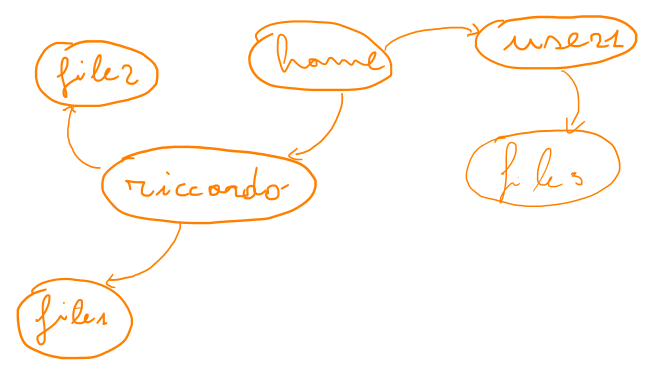
\includegraphics[width=15cm]{./immagini/whiteboard_sketch.png}
    \caption{Whiteboard sketch della struttura di un'ipotetica repository}
\end{figure}
Dopo aver creato il cosiddetto "whiteboard model" si procede alla formalizzazione delle entità e relazioni individuate, etichettando con label le entità e relazioni e associandovi tutte le proprietà.
\begin{figure}[H]
    \centering
    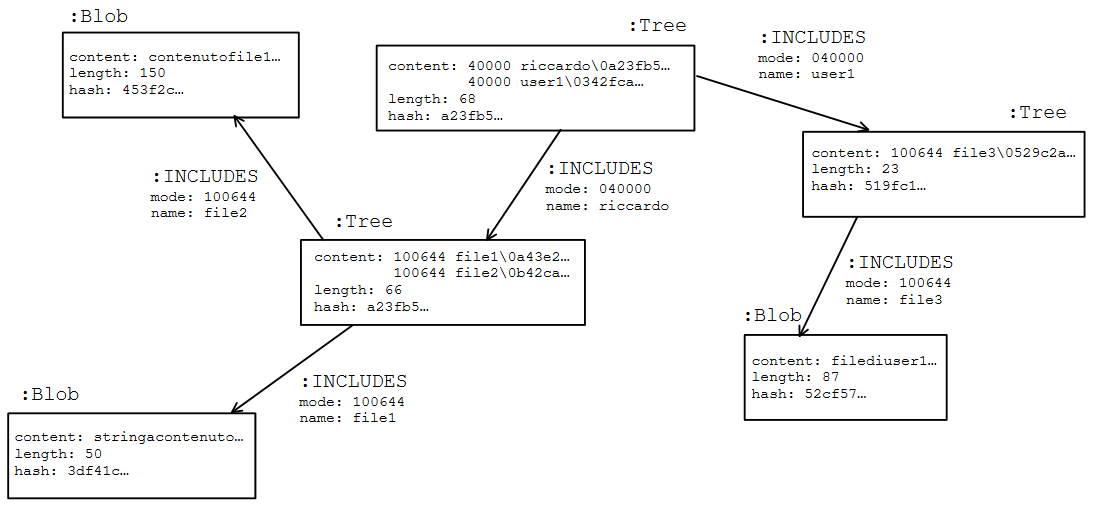
\includegraphics[width=15cm]{./immagini/whiteboard_formal.png}
    \caption{Formalizzazione dello sketch con proprietà e label}
\end{figure}
Come si nota dalla figura precedente si è deciso di assegnare i label (case sensitive) \texttt{:Tree} e \texttt{:Blob} alle rispettive entità, si individuano inoltre le seguenti proprietà per entrambi i tipi di oggetti:
\begin{itemize}
    \item \texttt{hash}: identificatore univoco dell'oggetto, calcolato con l'algoritmo SHA-1;
    \item \texttt{size}: dimensione in byte del contenuto;
    \item \texttt{content}: contenuto dell'oggetto, come descritti sopra.
\end{itemize}

Per le relazioni, in questo sottoinsieme del modello se ne individua soltanto una: il label \texttt{:CONTAINS} indica che oggetto ne contiene un altro. Le relazioni sono ordinate e nel caso di \texttt{:CONTAINS} il nodo di partenza è sempre un \texttt{:Tree} e il nodo di arrivo può essere sia un \texttt{:Tree} che un \texttt{:Blob}.
Si denotano inoltre due proprietà per questa relazione:
\begin{itemize}
    \item \texttt{name}: nome del file o della cartella;
    \item \texttt{mode}: GGit mode dell'oggetto, può assumere il valore "040000" se il nodo di arrivo ha il label \texttt{:Tree} e i valori {"100644", "100755", "120000"} se il nodo di arrivo ha il label \texttt{:Blob}.
\end{itemize}

È stata fatta la scelta di associare le proprietà \texttt{name} e \texttt{mode} alla relazione e non al nodo in quanto rispecchia correttamente il modello dei dati definito: un oggetto \texttt{blob}, così come un \texttt{tree}, non ha un nome o una mode associati fino al momento in cui viene inserito all'interno di un \texttt{tree}.

Sotto viene mostrato il whiteboard sketch relativo al modello dei \texttt{commit} e degli \texttt{user}, e come possono essere collegati tra di loro:
\begin{figure}[H]
    \centering
    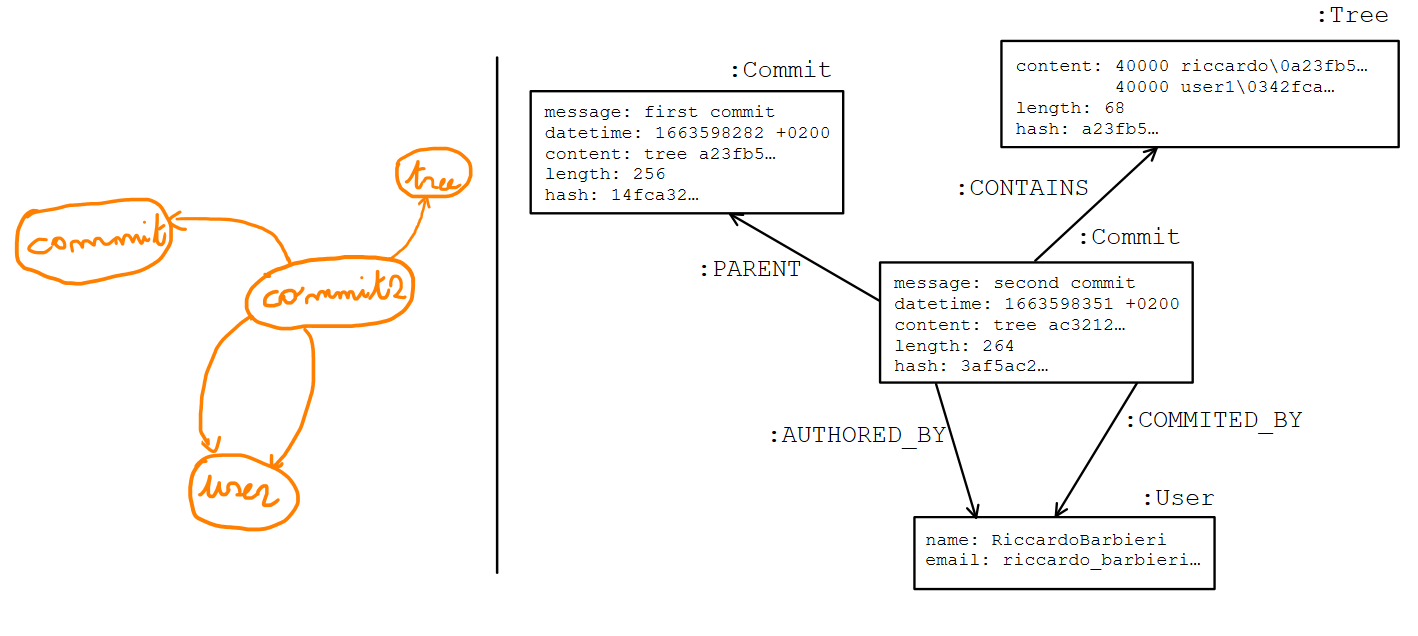
\includegraphics[width=15cm]{./immagini/whiteboard_commit.png}
    \caption{Whiteboard sketch del modello dei commit e degli user}
\end{figure}
In questa sezione del modello si individuano due nuove entità, \texttt{:Commit}, che è identificato dalle seguenti proprietà:
\begin{itemize}
    \item \texttt{message}: messaggio del commit;
    \item \texttt{datetime}: momento di creazione del commit (UNIX timestamp) e fuso orario (in ore dal UTC);
    \item \texttt{content}: stringa che rappresenta il commit (quella che viene data come input all'algoritmo di hashing).
    \item \texttt{length}: lunghezza del content.
    \item \texttt{hash}: identificatore univoco del commit, calcolato come descritto sopra;
\end{itemize}
Si identificano inoltre nuove relazioni: \texttt{:COMMITTED\_BY} e \texttt{:AUTHORED\_BY} che indicano rispettivamente il committer e l'autore di un commit; \texttt{:PARENT} che parte da un commit e punta al commit padre e infine \texttt{:CONTAINS} che parte da un commit e punta ad un oggetto \texttt{tree} che rappresenta lo stato della repository al momento del commit.
Si denota infine l'entità \texttt{:User}, identificata dalle seguenti proprietà:
\begin{itemize}
    \item \texttt{name}: nome dell'utente;
    \item \texttt{email}: email dell'utente;
\end{itemize}

Come dimostrato, il modello whiteboard è estremamente utile per formalizzare le entità e relazioni in gioco e per individuare le proprietà da associare ad esse, data la natura ad alto livello di questo approccio è molto semplice passare da un idea, o uno sketch, a una definizione formale del modello dei dati.
\section{Interfaccia utente}
\section{Impostazioni di configurazione}
\section{Manager}
\subsection{Difference}
\subsection{Stash}
\subsection{Neo4j}
%! comandi

%! configurazioni

%! difference manager (no implementation)

%! stash manager (no implementation)

%! neo4j manager